\documentclass[11pt, cleanfoot, cleanhead]{asme2e}
\usepackage{hyperref, eurosym, wrapfig, graphicx, textcomp, ragged2e, booktabs, amssymb,mathtools, multicol, incgraph,tikz,subcaption}
\usepackage[export]{adjustbox}
\newcommand*{\coverPage}{\begingroup% Gentle Madness 

\incgraph[documentpaper][width=\paperwidth,height=\paperheight]{./figures/cover.png}
\clearpage
\endgroup}
\providecommand{\versionnumber}{1.1}


\title{BlockLicense: A Decentralized Ecosystem for Licensing \& Funding}  
\author{ The BlockLicense Team 
    \affiliation{
		BlockLabs P.C.\\
		Leof. Andrea Siggrou 190\\
		Kallithea, 17671, Greece\\ 
		Email: info@blocklicense.io
    }
}
\hypersetup{pdfinfo={
Title={BlockLicense: A Decentralized Ecosystem for Licensing \& Funding},
Author={The BlockLicense Team},
Subject={BlockLicense Whitepaper v\versionnumber},
Keywords={BlockLicense, Whitepaper, Licensing, Funding, Creative Industry, License Coin, LCN, Cryptocurrency},
Producer={LaTeX},
Creator={pdflatex}
}}
\begin{document}
\coverPage
\pagenumbering{arabic}
\maketitle    
\bigskip
\begin{center}
\textbf{This is not a consultation for investment paper and it should not be considered as one.}
\end{center}
\bigskip
\begin{abstract}
{\it BlockLicense is a decentralized ecosystem that enables fair licensing, pricing and distribution of creative content and aims to liberate creators from intermediates. BlockLicense has licensing, pricing and attribution at its very core by embedding relevant information to the backbone of digital files without altering their behavior. Transactions within BlockLicense take place through an ecosystem-specific coin, namely the License Coin (LCN) that is based on Ethereum and is compatible with smart contracts running on the Ethereum Virtual Machine. Distributed file systems and databases are used for file storage and information retrieval. The BlockLicense ecosystem is a complete solution that provides plugins for popular design software, enabling creators to add licensing and pricing to their creative workflow, a desktop application, a browser extension, as well as a web-based platform where end-users can easily acquire a license for their required content. We believe that BlockLicense is a revolutionary project that can completely alter the way creative work is distributed and funded and can have a positive impact on both creators and buyers.}
\end{abstract}
\begin{nomenclature}
\entry{EVM}{Ethereum Virtual Machine}
\entry{ETH}{Ether}
\entry{LCN}{License Coin}
\end{nomenclature}

\section{INTRODUCTION} \label{introduction}

 Technological advances such as the broadband internet, powerful computers, mobile devices with exceptional cameras, improved and intuitive design software as well as widely available online tutorials have lowered the barrier and most people with basic technological  literacy can become creators of digital work. Every single day more than 1.1 trillion digital files such as audio, photographs, videos, documents, ebooks and design files are created. 90\% of world's data was created in the last two years alone \cite{ibm}. 

The Web is the ideal medium that allows creators to reach a worldwide audience and sell their work while being able to sustain themselves. In practice though, this is far from reality. Current channels for content licensing and monetization fail to provide creators the freedom to decide how to license and distribute their work and usually, the monetary compensation for work sold is severely reduced due to large fees applied on sales.

At BlockLabs we believe that blockchain and specifically the Ethereum \cite{buterin2013ethereum} Blockchain and Virtual Machine offer the ideal medium on which a system for fair content licensing and monetization can be built. The Ethereum blockchain is public, distributed and immutable and enables the creation of arbitrary paying systems and structures while maintaining overall security. Also, it enables very fast transaction processing times, it has low fees and it is borderless. The Ethereum blockchain and virtual machine, provide the building blocks for an ecosystem of tools and services that can revolutionize the way digital content is licensed, distributed and sold.

BlockLicense is a project that aims to provide creators with all the tools that can make licensing an integral part of their creative workflow and provide buyers with several avenues to discover and license fairly-traded digital content. The BlockLicense Ecosystem is designed from the ground up with Licensing at its very core and can accommodate a wide range of licensing scenarios such as ones where only one creator is involved, to more complex ones with multiple stakeholders. 

\section{MARKET LANDSCAPE} \label{landscape}
During 2016 alone, an estimated 1.61 billion people purchased goods online and global e-retail sales amounted to \$1.9 trillion. In Asia Pacific, online sales accounted for 12.1\% of retail sales, but only 1.8\% in the Middle East and Africa. Projections on market growth, estimate a growth of up to \$4.06 trillion by 2020. These projections are based on global buying trends driven by millennials, on  GDP forecasts  driven by certain geographies and web-related industries, growth on emerging markets such as Africa, predicting a large number of new internet users added to the global market pool, becoming decisive for future online sales.
 
Global statistics reveal that purchase intention rates among online shoppers vary strongly by product category - as we can see in Figure \ref{fig:file_categories}, 50\% of online purchases involve books (hard copies \& eBooks) and music . The average number of annual online transactions per capita is not uniform - Asian buyers account for an average of 22.1\% of online transactions, whereas buyers in Latin America represent a 9.2\%. 

The online digital files market is rapidly expanding and as we can see in Figure \ref{fig:market}, it is expected to double in size over the next two years. As the market expands, a multitude of distribution channels exist for creators to sell their digital content. 

\begin{figure}[!bp]
\centering
\begin{minipage}{.5\textwidth}
  \centering
  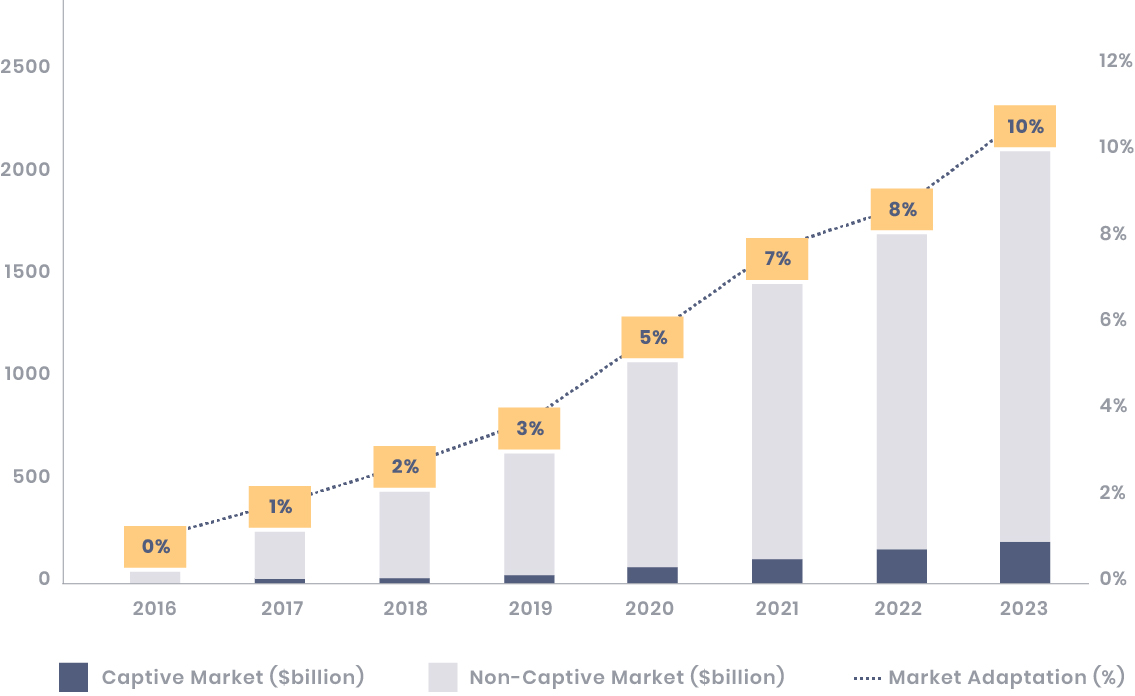
\includegraphics[width=0.8\linewidth]{./figures/fig1.jpg}
  \captionof{figure}{Online digital files market ( \$billion )}
  \label{fig:market}
\end{minipage}%
\begin{minipage}{.5\textwidth}
  \centering
  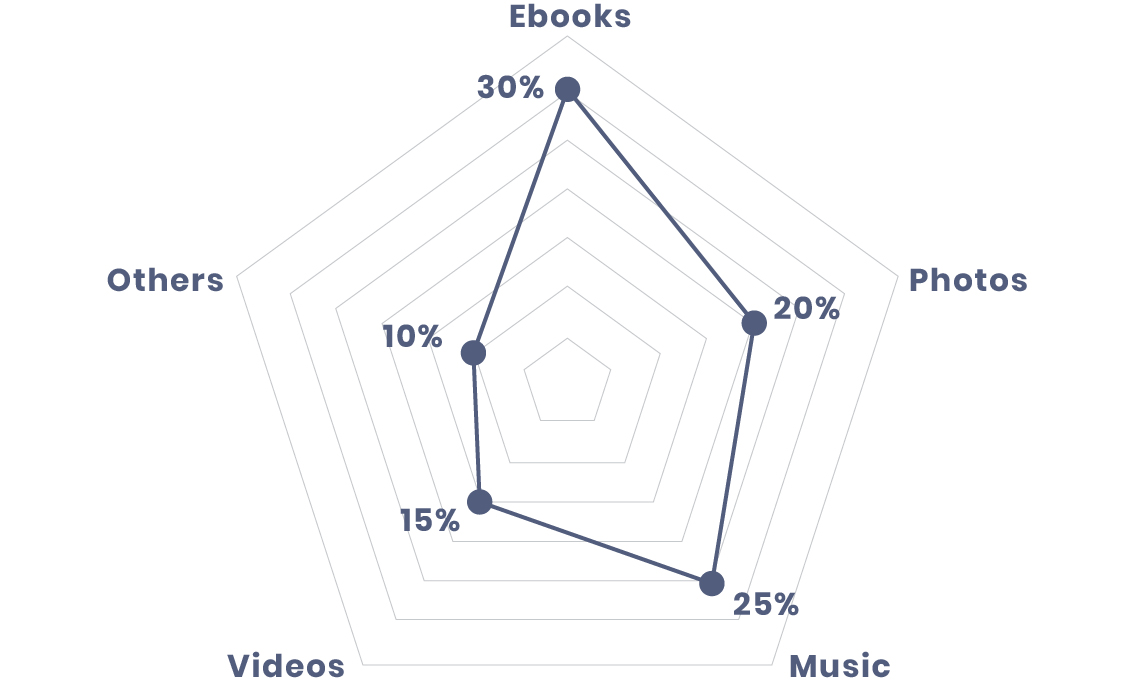
\includegraphics[width=0.8\linewidth]{./figures/fig2.jpg}
  \captionof{figure}{Digital file categories sales}
  \label{fig:file_categories}
\end{minipage} 
\end{figure}


The main distinction among current offerings is whether the solution used facilitates a direct connection between the creator and the buyer or it enables the creator to reach a wider audience without facilitating a direct sell. Using industry terms, the two main offerings are known as Maker Platforms and Exchange Platforms and in the following section we will review their advantages and shortcomings.
The online digital files market is rapidly expanding and as we can see in Figure \ref{fig:market}, it is expected to double in size over the next two years. Among the types of files that are sold online, Ebooks and music account for over 50\% of the sales ( Figure \ref{fig:file_categories} ). 
 


%%%%%%%%%%%%%%%%%%%%%%%%%%%%%%%%%%%%%%%%%%%%%%%%%%%%%%%%%%%%%%%%%%%%%%
\subsection{Maker Platforms}

Several stock content websites exist where creators can fully give up their licensing and pricing rights and get a commission on copies of work sold. Such websites do not require a subscription by the creator but are customer centric and provide subscription plans for end users. Submitted work needs to go through a thorough vetting process before it is included in the catalog of works available. Such websites theoretically offer a lot of visibility since they tend to have a huge user base but, in practice, ones work can easily be lost among the myriad of similar offerings. As we can see in Table \ref{comp-matrix} creators only receive a small fraction of the retail price of their work, buyers need to have a valid paid subscription and creators have no control over the licensing and pricing of their work.


%%%%%%%%%%%%%%%%%%%%%%%%%%%%%%%%%%%%%%%%%%%%%%%%%%%%%%%%%%%%%%%%%%%%%%

\subsection{Exchange Platforms}

Exchange platforms enable creators to facilitate a direct sell by providing an inventory, payment processing, shopping cart and cloud based storage as a service. Such offerings usually require a time-based subscription by the creator and display product listings either in a central website or provide embeddable widgets that creators can use to display and sell their products through their own website. While Exchange Platforms give full control to creators over the licensing and pricing of their work, as we can see in Table \ref{comp-matrix} they are charged a fee on work sold and an active paid subscription is required.
\newline
\bigskip

\subsection{BUSINESS MODEL} \label{businessmodel}

Both solutions as described above, have a centralized nature and impose great restrictions to Creators and Buyers.

BlockLicense introduces a new business model that puts Creators and Buyers at the forefront by removing all restrictions imposed by Maker and Exchange Platforms and by  providing tools that simplify the licensing process and allow a wide range of licensing scenarios. Payment processing and routing as well as proof-of-ownership is automated with Ethereum smart contracts.

Multiple channels of distribution are provided including a Web Platform, website embedded shops \& offline distribution of files. All transactions and payouts within BlockLicense are instant while both creators and buyers are free of subscription or hidden costs. A flat 2\% fee is imposed in all transactions to cover BlockLicense costs and allow a continuous and organic expansion of the ecosystem.

\begin{figure}[bp]
\centering
\begin{minipage}{.45\textwidth}
  \centering
  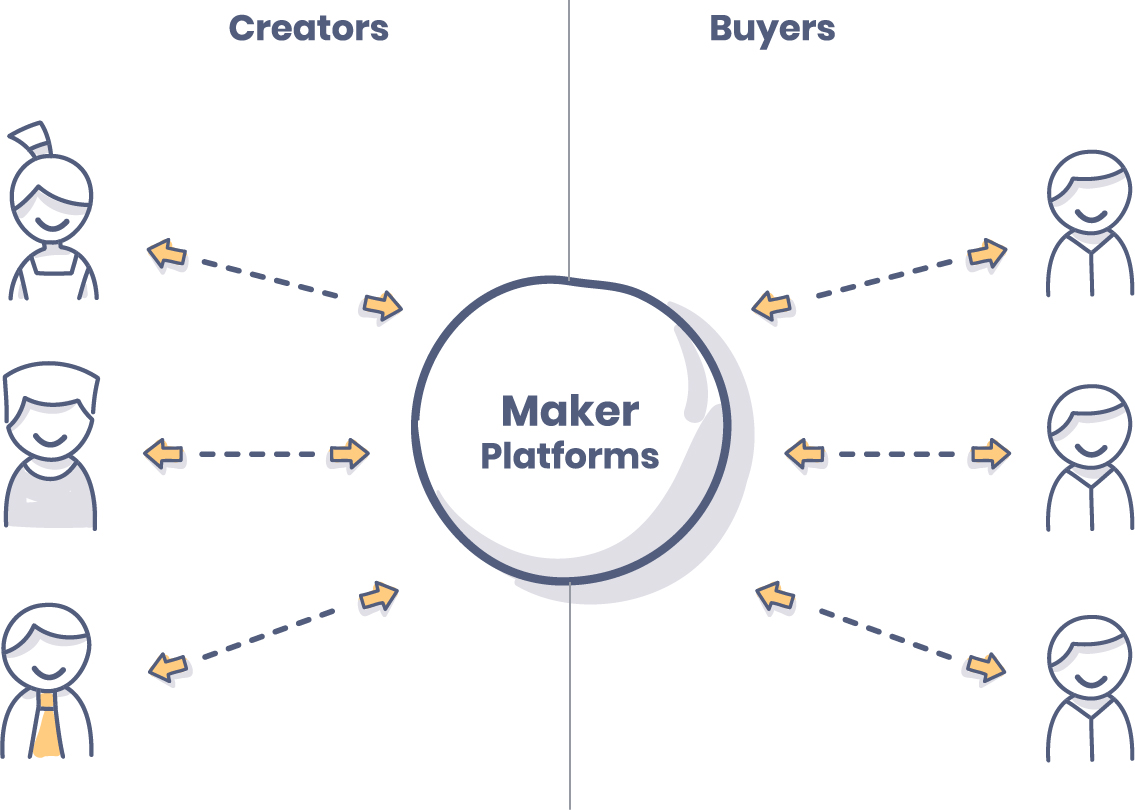
\includegraphics[width=.8\linewidth]{./figures/fig9.jpg}
  \captionof{figure}{Maker Platforms.}
  \label{fig:maker}
\end{minipage}
\begin{minipage}{.45\textwidth}
  \centering
  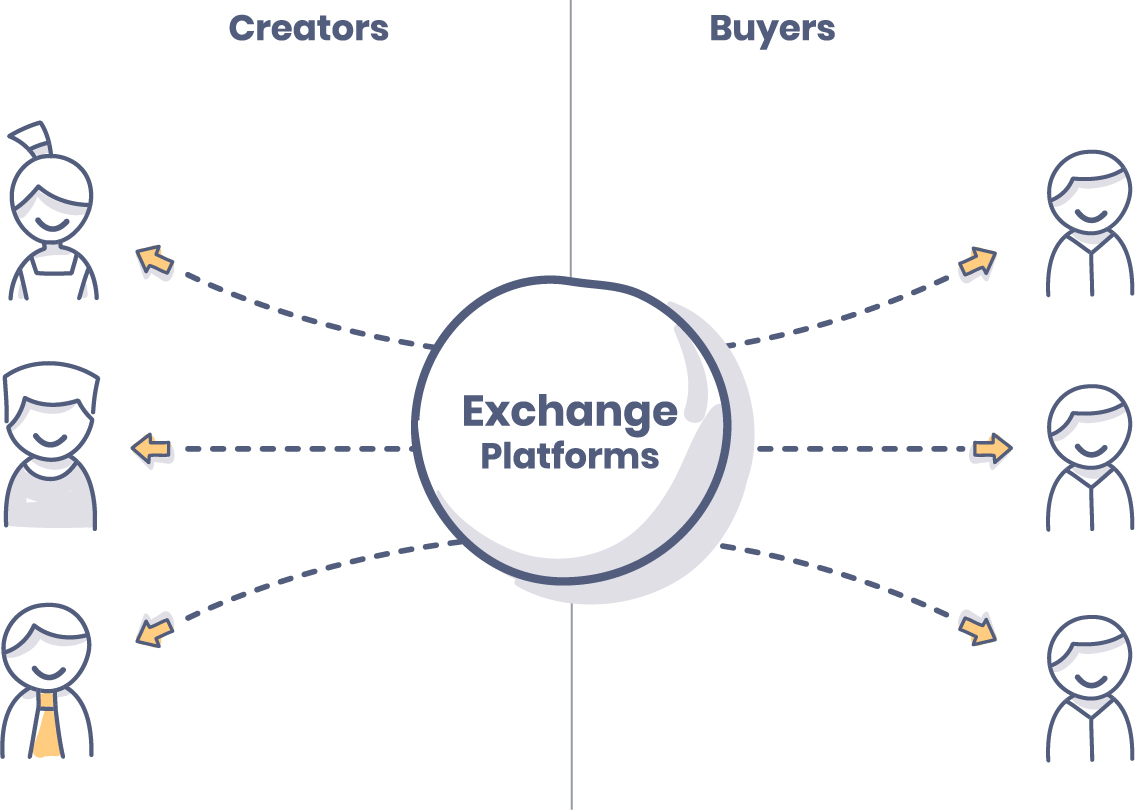
\includegraphics[width=.8\linewidth]{./figures/fig10.jpg}
  \captionof{figure}{Exchange Platforms.}
  \label{fig:exchange}
\end{minipage}%
\end{figure}


%%%%%%%%%%%%%%%%%%%%%%%%%%%%%%%%%%%%%%%%%%%%%%%%%%%%%%%%%%%%%%%%%%%%%%
\clearpage
\section{LICENSING} \label{licensing}

Licensing is the cornerstone of BlockLicense. It takes place with specialized software that embeds licensing \& pricing information within the file itself.  The Creator sets information about the work such as:

\begin{description}
\item[Creator Info:] Attribution details about the creator 
\item[Project Info:] Information related to the project such as name and description
\item[Licensing:] Licensing and pricing options for the project
\end{description}

It is important to note that the process of embedding attribution and licensing information within the file doesn\textquotesingle t alter the way the file works and that  once the BlockLicense data is embedded, it follows the file throughout its lifetime, whether on-line or off-line. As we can see in Table \ref{table:filetypes}, a wide range of filetypes is supported out of the box, while additional popular filetypes will be supported in the future. 

% Please add the following required packages to your document preamble:
% \usepackage{booktabs}
\begin{table}[t]
\centering
\begin{tabular}{@{}rl@{}}
\toprule
\multicolumn{1}{l}{}             & \multicolumn{1}{c}{\textbf{BlockLicense Compatible Filetypes}}         \\ \midrule
\textbf{Video}                   & WMV, FLV, AVI, MOV, MPEG-4, SWF, AVCHD, P2, Sony HDV, XDCAM \\
\textbf{Audio}                   & WMA, AIFF, WAV, MP3, MPEG-2                                 \\
\textbf{Photo}                   & JPEG, JPEG2000, DNG, PNG, BMP, TIFF, GIF                    \\
\textbf{Vector}                  & SVG, EPS, PS, PDF, AI                                       \\
\textbf{Document}                & PDF, PS, EPS, UCF                                           \\
\textbf{Digital Design Software} & AI,  PSD, INDD, INDT                                        \\ \bottomrule
\end{tabular}
\caption{The initial set of filetypes supported by BlockLicense.}
\label{table:filetypes}
\end{table}

\subsection{OpenLicense}

At BlockLabs we are strong supporters of Open Source and believe that Open Source work deserves promotion and visibility that can allow creators to sustain themselves and support their work. Although the Open Source movement started in the 80s with a focus on computer source code, it has greatly expanded and includes many categories such as software, design and hardware. Nowadays, Open Source can be found everywhere and is used on a daily basis by users that often do not realize that they use something that was built by collaborating creators over the Internet and distributed for free. Notable examples include Firefox \cite{firefox}, MySQL \cite{mysql}, Android \cite{android}, Linux \cite{linux}, Wordpress \cite{wordpress}, VLC \cite{vlc} and Kodi \cite{kodi} to name a few.

Although Open Source work is free to use, as long as licensing terms are met, no de--facto standard exists that enables end-users to support Open Source projects via donations. With OpenLicense we aim to standardize the way Open Source projects are funded by enabling creators to attach an Open Source license to their work and accept donations.

A creator gets to choose the desired license from a preloaded set of standard Open Source licenses such as the BSD licenses \cite{bsd}, GNU GPL \cite{gpl}, the Apache Licenses \cite{apache}, the MIT license \cite{mit}, Creative Commons  licenses \cite{cc} and so on, or set his/her own license and accept donations. 
 
\begin{figure}[!b]
\centering
\begin{minipage}{1\textwidth}
  \centering
  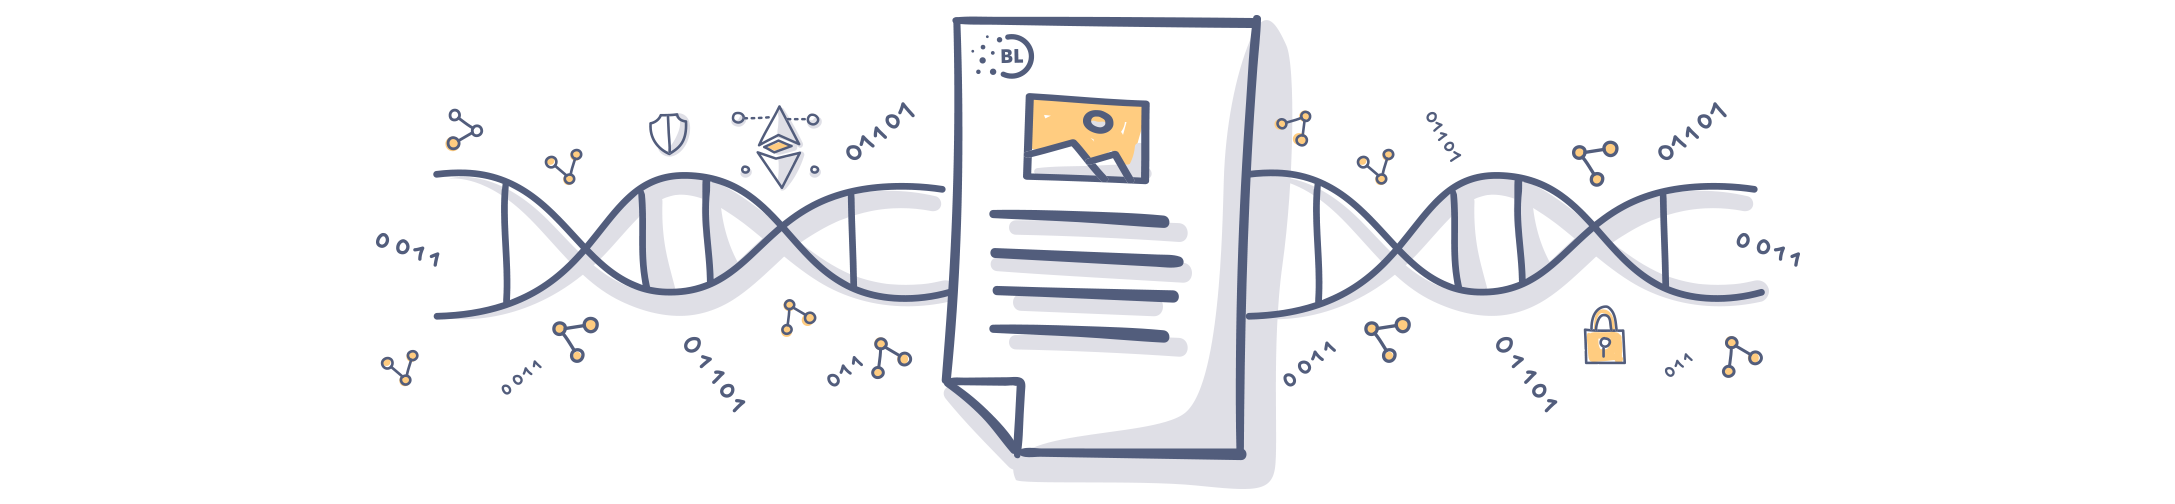
\includegraphics[width=1\linewidth]{./figures/fig3.png}
  \caption{Embedding licensing \& pricing data to file.}
  \label{fig:licensing}
\end{minipage}%
\end{figure}
\begin{figure}[!t]
\centering
\begin{minipage}{1\textwidth}
  \centering
  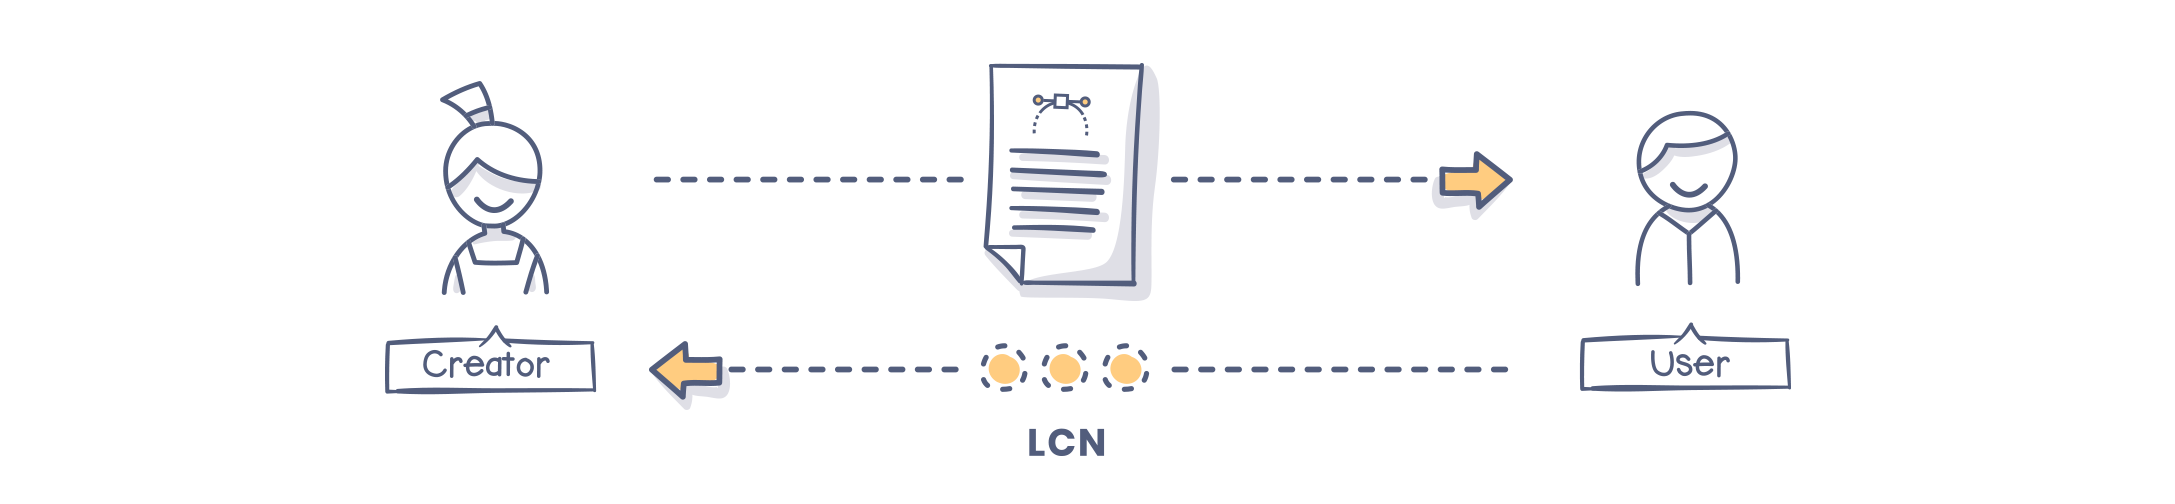
\includegraphics[width=1\linewidth]{./figures/fig4.png}
  \caption{Accepting donations for Open Source files.}
  \label{fig:donations}
\end{minipage}
\end{figure}


%%%%%%%%%%%%%%%%%%%%%%%%%%%%%%%%%%%%%%%%%%%%%%%%%%%%%%%%%%%%%%%%%%%%%%

\subsection{ClosedLicense}

ClosedLicense corresponds to all commercial licenses that require a fee. In contrast to OpenLicense where one can only fund a project via a donation, ClosedLicense doesn't support donations but supports more complex licensing scenarios such as \textit{multiple stakeholders}, \textit{multiple licenses} and \textit{reselling}.

As shown in Figure \ref{fig:stakeholders} a ClosedLicense work can have multiple stakeholders with different stakes on work produced ( e.g in the case of music, different members of a band, a producer and so on). By defining the set of stakeholders of a project and the respective percentage each stakeholder should receive when the work is sold, the process of sharing profit is streamlined. Everytime the work is sold, ClosedLicense makes sure that funds are almost instantly distributed to corresponding stakeholders using the specified percentages that were set when the digital file was introduced in the BlockLicense Ecosystem.

\begin{figure}[h]
\centering
\begin{minipage}{1\textwidth}
  \centering
  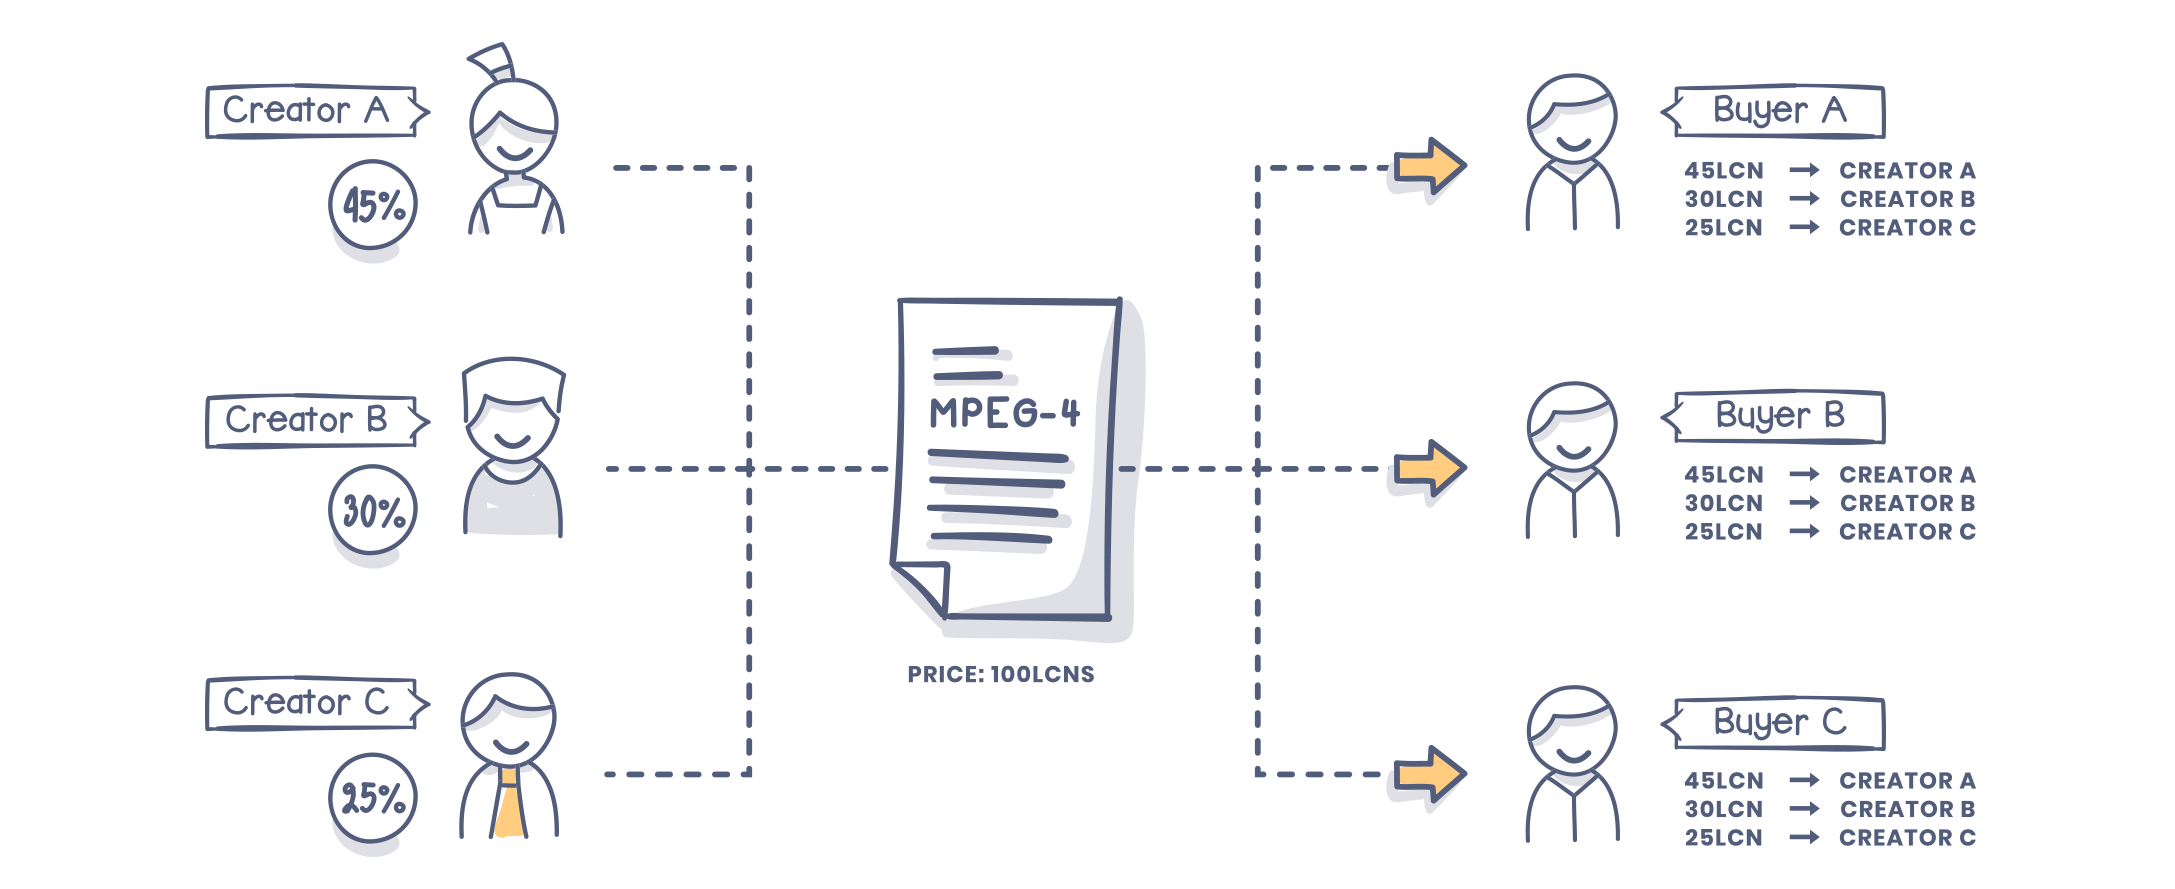
\includegraphics[width=1\linewidth]{./figures/fig5.png}
  \caption{Multiple stakeholders.}
  \label{fig:stakeholders}
\end{minipage}
\end{figure}

ClosedLicense supports different licensing schemes for different use cases for the same piece of work. As an example let's consider a photographer that wants to release his/her work using BlockLicense. He/she can set a different pricing for a photograph to be used in a non-commercial website, a commercial site, for print and so on.

As shown in Figure \ref{fig:reselling} ClosedLicense allows creators to enable Reselling and set a reseller fee. By doing so, creators essentially turn all buyers of their work into potential resellers, geometrically expanding their distribution network. This is advantageous to both creators and buyers since creators get greater visibility and potentially an increase in sales while buyers can get an income on work resold.

\begin{figure}[h]
\begin{minipage}{1\textwidth}
  \centering
  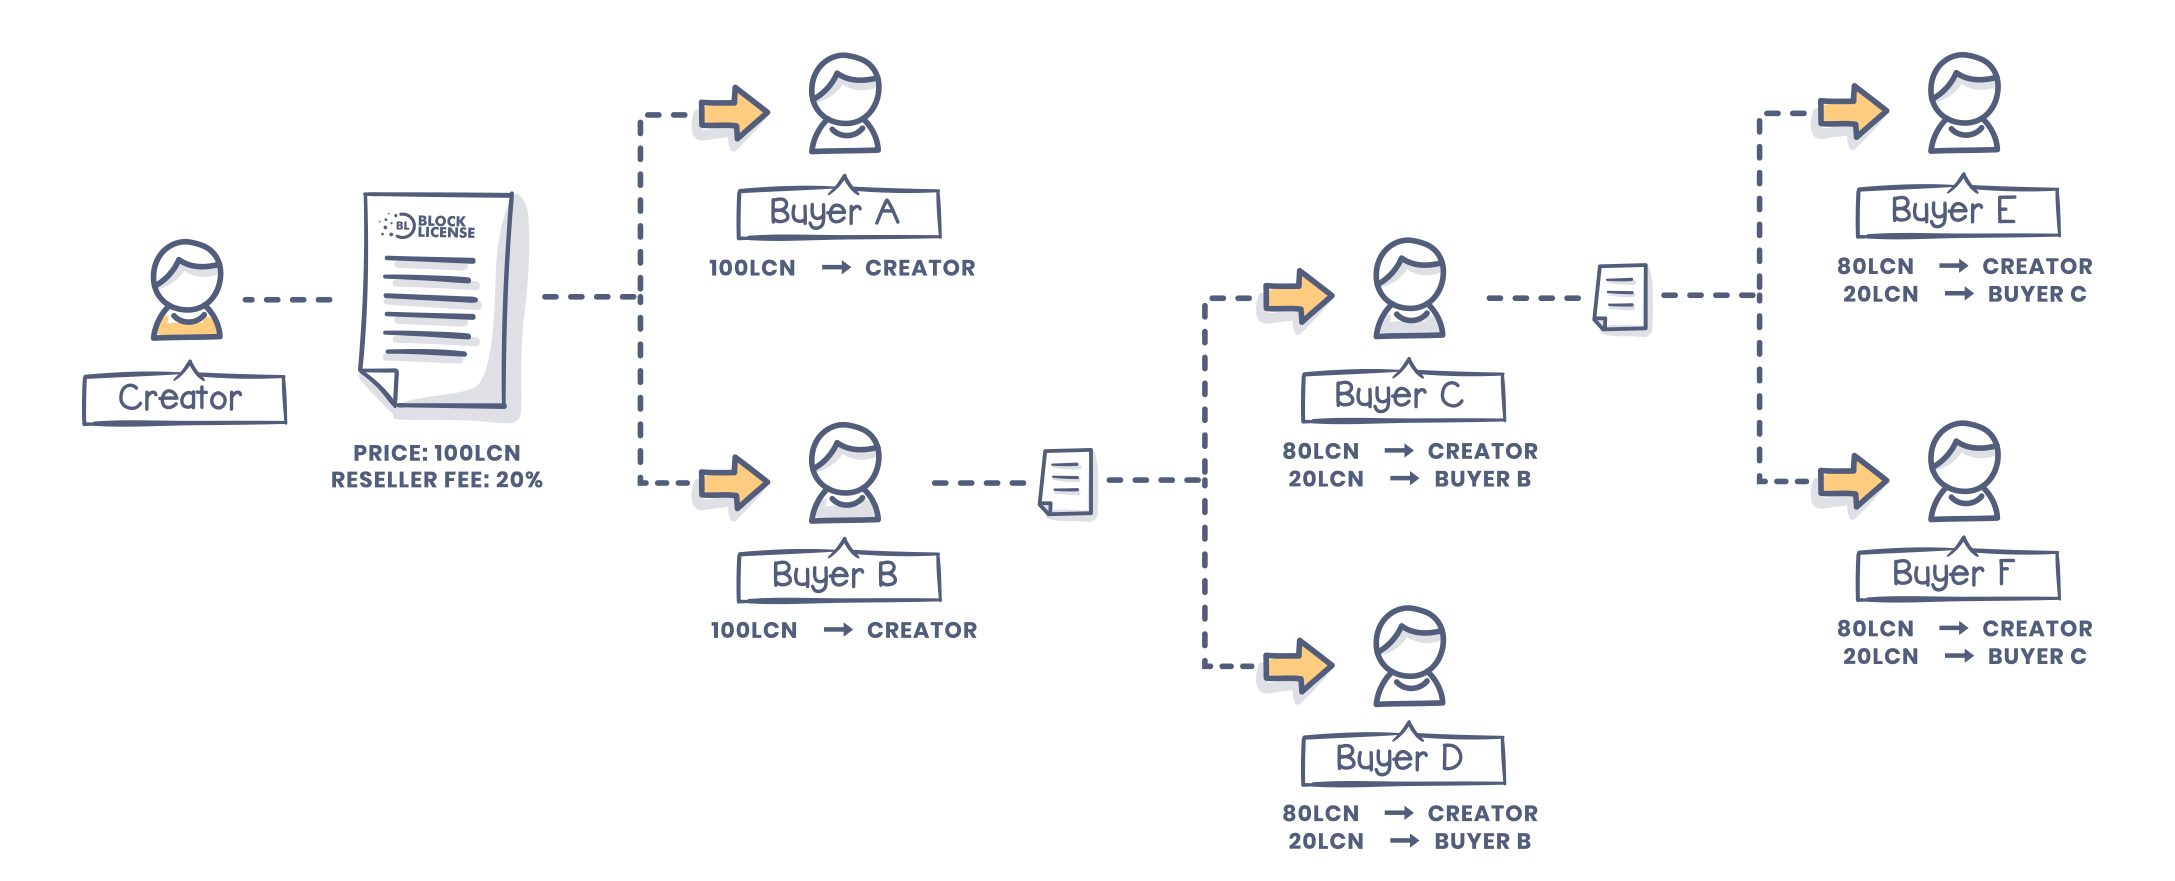
\includegraphics[width=1\linewidth]{./figures/fig6.png}
  \caption{Reselling of files.}
  \label{fig:reselling}
\end{minipage}
\end{figure}

\section{ECOSYSTEM} \label{ecosystem}

We believe that the current model of Maker \& Exchange Platforms is not fair to creators and buyers and that by using decentralized systems where no central authority has control, we can build an ecosystem of tools \& services that offers creators the freedom to license \& distribute their work, while maintaining all benefits of existing traditional platforms. The BlockLicense ecosystem aims to embrace both creators and buyers and make the process of licensing \& funding extremelly simple by providing a wide range of tools specifically created for this purpose.


\subsection{The License Coin}

All transactions within the BlockLicense ecosystem take place in License Coins (LCN) (Table \ref{table:lcn}), an Ethereum based ERC20 \cite{erc20} token, enabling very fast transactions and almost instant payouts. An ecosystem-specific token is paramount to the viability of the project since its price is not affected by the fluctuations of Ether, it creates a closed ecosystem economy and it enables us to provide incentives to creators and buyers for participating in the BlockLicense Ecosystem. Also, since LCN has utilitarian value within the BlockLicense ecosystem, LCN holders will be encouraged to use BlockLicense for their licensing needs and help the community grow. Initial LCN distribution will take place through a crowdsale that is described in detail in Section \ref{crowdsale} of this document and through which we will be bootstrapping the development and promotion of the ecosystem. Once the LCN crowdsale is over, LCN will be listed in several crypto exchanges to be traded at will.

\begin{table}[t!]
\begin{center}
\begin{tabular}{c c c c c c}
& & \\ % put some space after the caption
\toprule
\textbf{Name} & \textbf{Symbol}  & \textbf{ETH Rate} & \textbf{Total Issued}  & \textbf{Decimal Points} & \textbf{Type}\\
\midrule
 License Coin & LCN & 2,000 LCN to 1 ETH & 700,000,000 LCN & 18 & ERC20\\
\bottomrule
\end{tabular}
\end{center}
\caption{License Coin Data}
\label{table:lcn}
\end{table}

\subsection{The Web Platform}

The BlockLicense Web Platform is a web-based marketplace for BlockLicense content. The Platform is the central gateway where buyers can browse submitted content and acquire licenses on digital files for their desired use-case. The Web Platform is mainly targetting buyers of digital content.

\subsection{Website Shop Widgets}
A very important part of the ecosystem are Shop Widgets that enable the embedding of shops in custom websites. Shop widgets utilize the Reseller feature of BlockLicene, by enabling buyers to act as curators of content and create lists of digital content than can be embedded and sold through their personal websites.

\subsection{The BlockLicense App}

The BlockLicense Desktop App is a cross-platform application available in all major Operating Systems (Windows, OSX, Linux) targeting both creators and buyers. It acts as a software-based LCN wallet that enables token holders to transfer Lisense Coins, view licensing information of local files that have the BlockLicense information embedded and acquire licenses for permissible uses. Creators can use the application to manage their cloud-based library of custom licenses, add BlockLicense information to their files by setting their desired licensing and pricing options and submit their content to the BlockLicense Web Platform. The Desktop Application integrates fully with the rest of the ecosystem and provides one of the main pathways users can take to produce and consume BlockLicense content.

\subsection{Design Software Plugins}

With BlockLicense we aim to make the process of setting licensing \& pricing information very simple and make sure it does not add significant work to creators. By creating BlockLicense plugins for popular design software such as ones created by Adobe \cite{adobe}, we aim to make the process of licensing an integral part of the creators workflow, all within a familiar environment. Complex tasks such as optimal pricing determination can be greatly simplified by providing usefull feedback to creators such as the average price of similar work and the price of bestseller items within the ecosystem. Design software plugins integrate with the rest of the ecosystem and allow creators to set their licensing \& pricing options and make their files available within the Web Platform.



\subsection{Mobile App}

The BlockLicense MobileApp provides tools for submitting time-sensitive content such as footage \& photos of events that are newsworthy. It connects people on the streets with newsrooms and integrates with the Web Platform so that news networks can acquire licenses for their desired content. It enables citizen journalists to sell their content and provides breaking news videos \& photos to news networks.


\subsection{BlockLicense Architecture}

The BlockLicense Architecture utilizes decentralized services for the core functionality of the system, enforcing the longevity of submitted data while decoupling the availability of services from BlockLicense success. The Ethereum blockchain and Virtual Machine are used for the verification of all BlockLicense metadata attached to a file and for all payment processing and routing needs as specified by the creator. IPFS \cite{ipfs} is used for storage of binary files while BigchainDB \cite{bigchaindb} is used for all database related needs of the ecosystem.

\begin{figure}[h]
\centering
\begin{minipage}{1\textwidth}
  \centering
  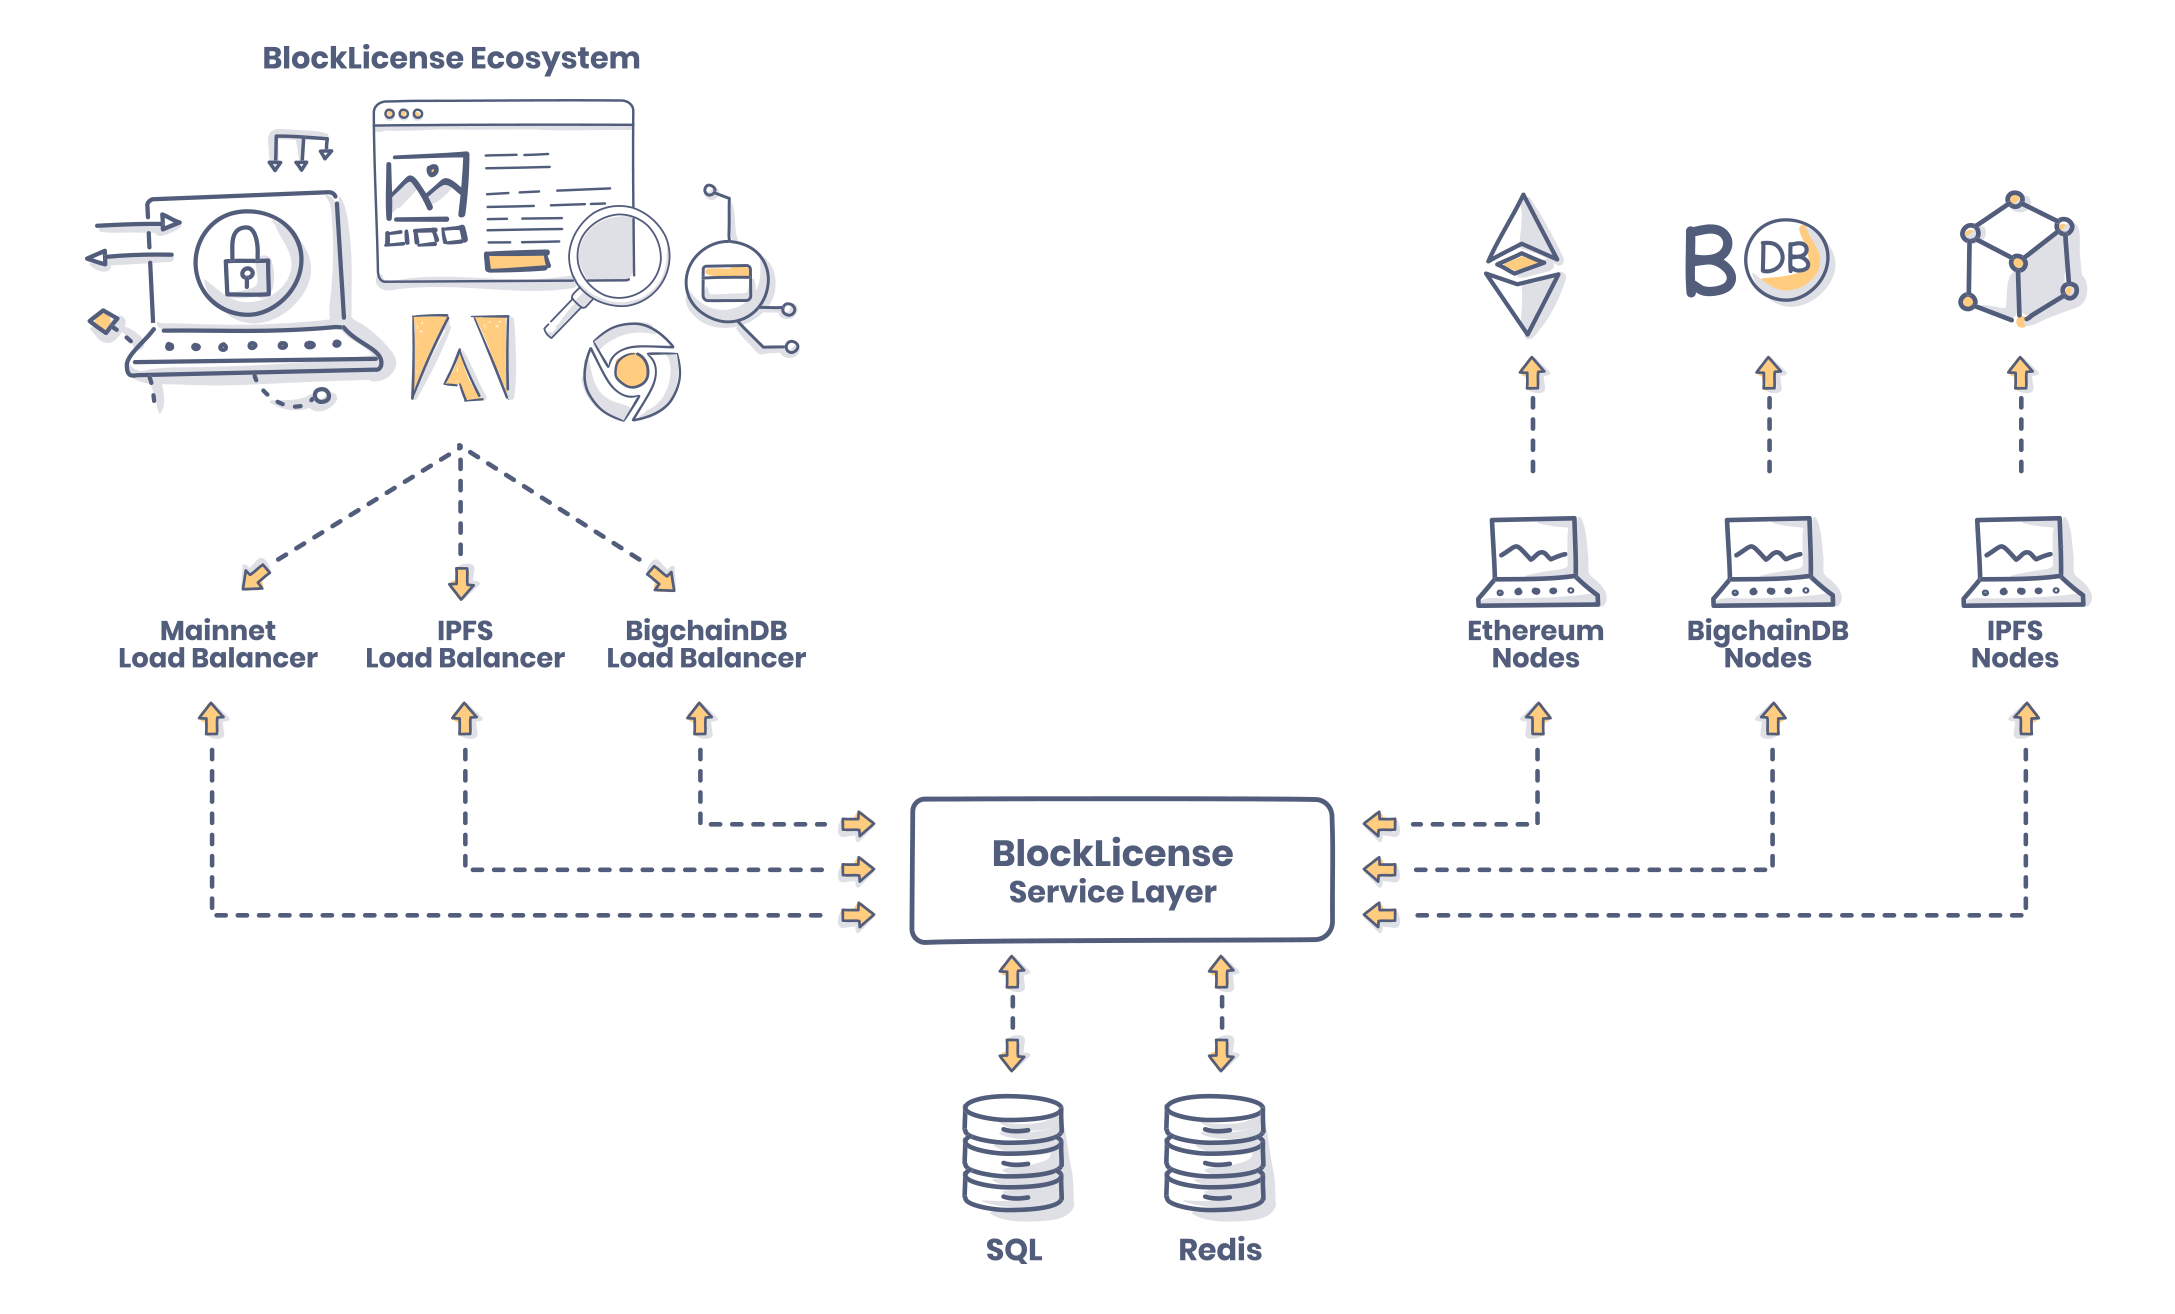
\includegraphics[width=1\linewidth]{./figures/fig7.png}
  \caption{BlockLicense System Architecture.}
  \label{fig:system}
\end{minipage}%
\end{figure}

\newpage
\section{ROADMAP} \label{roadmap}

The BlockLicense project has gone a long way since the initial concept was formed in the beginning of 2017. 

\begin{figure}[h]
\centering
\begin{minipage}{1\textwidth}
  \centering
  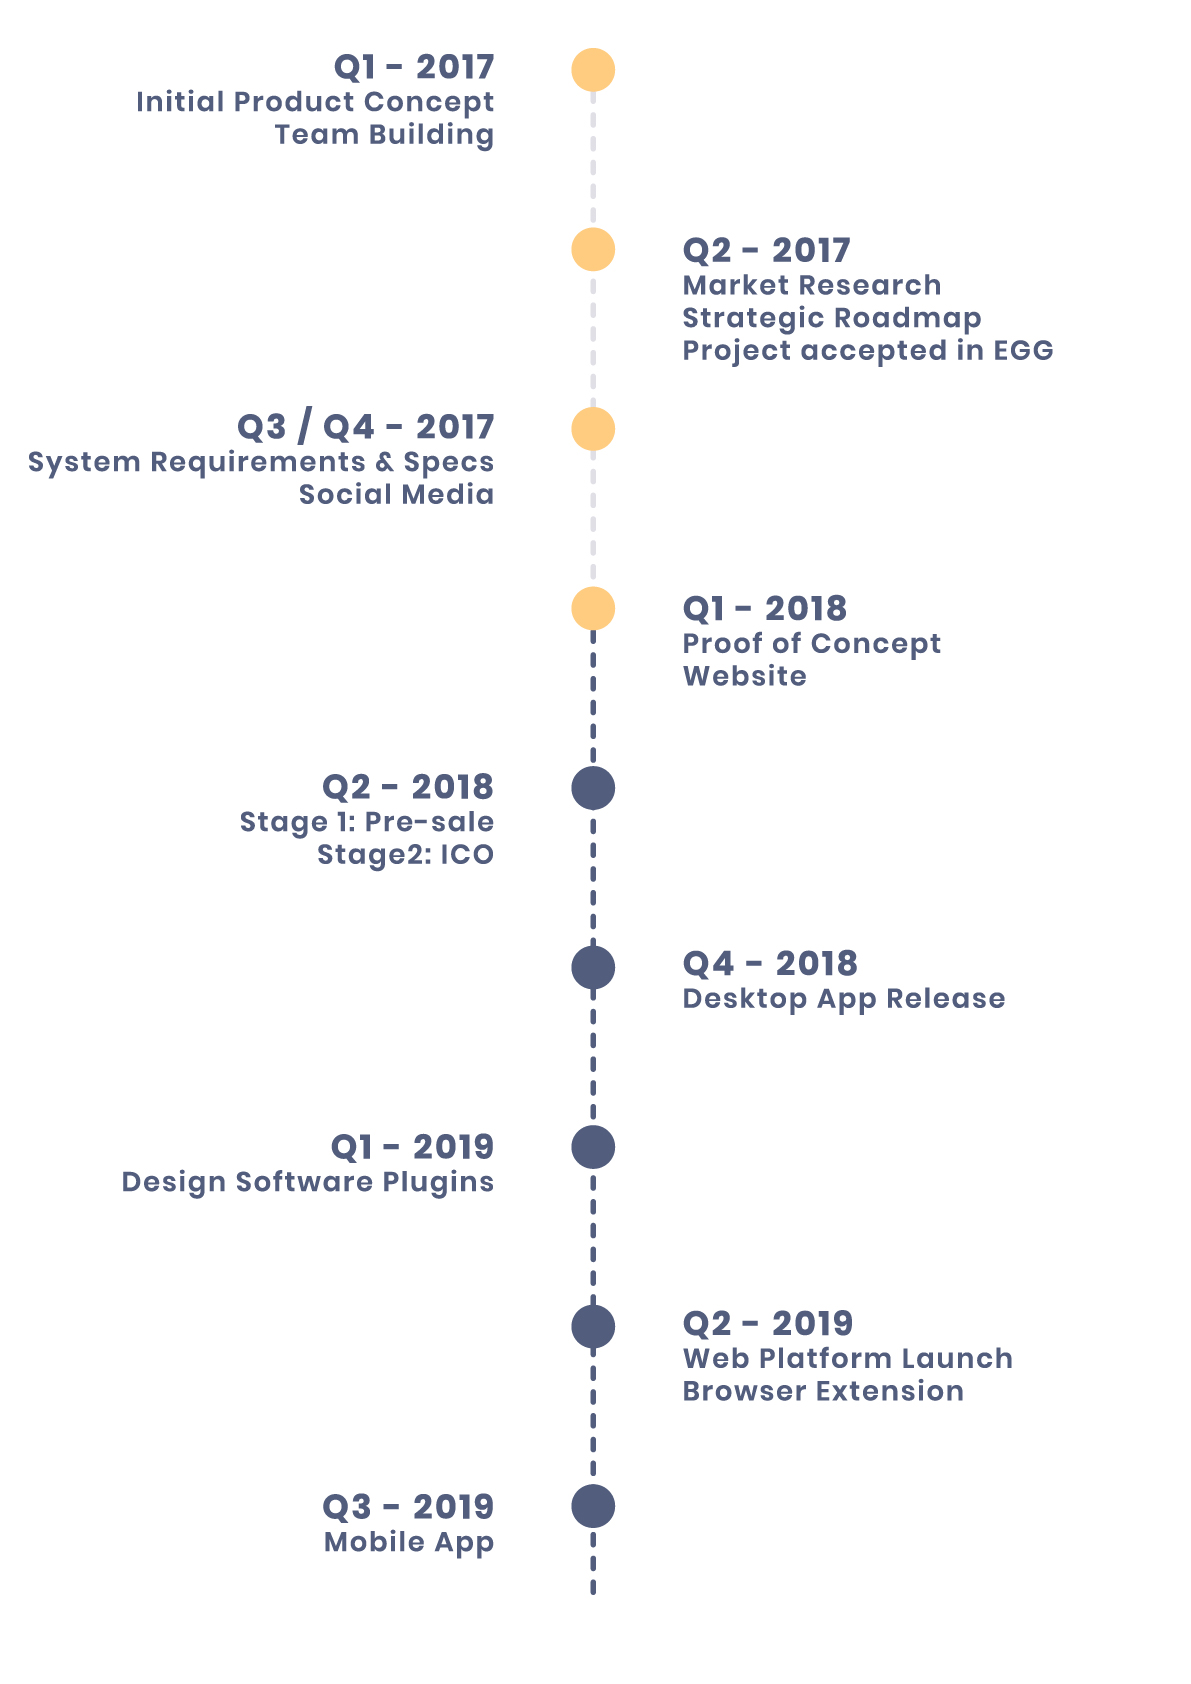
\includegraphics[width=.65\linewidth]{./figures/fig8.jpg}
  % \caption{figure}{The BlockLicense Roadmap.}
  % \label{fig:roadmap}
\end{minipage}%
\end{figure}
\newpage
\section{BUSINESS MODEL} \label{businessmodel}

As we described in Section \ref{landscape}, the online digital content market can be grouped in two major business models, namely Maker and Exchange Platforms. Both solution have a centralized nature and impose great restrictions to Creators and Buyers.

BlockLicense introduces a new business model that puts Creators and Buyers at the forefront by removing all restrictions imposed by Maker and Exchange Platforms and by  providing tools that simplify the licensing process and allow a wide range of licensing scenarios. Payment processing and routing as well as proof-of-ownership is automated with Ethereum smart contracts.

Multiple channels of distribution are provided including a Web Platform, website embedded shops \& offline distribution of files. All transactions and payouts within BlockLicense are instant while both creators and buyers are free of subscription or hidden costs. A flat 2\% fee is imposed in all transactions to cover BlockLicense costs and allow a continuous and organic expansion of the ecosystem.

\begin{figure}[h]
\centering
\begin{minipage}{.45\textwidth}
  \centering
  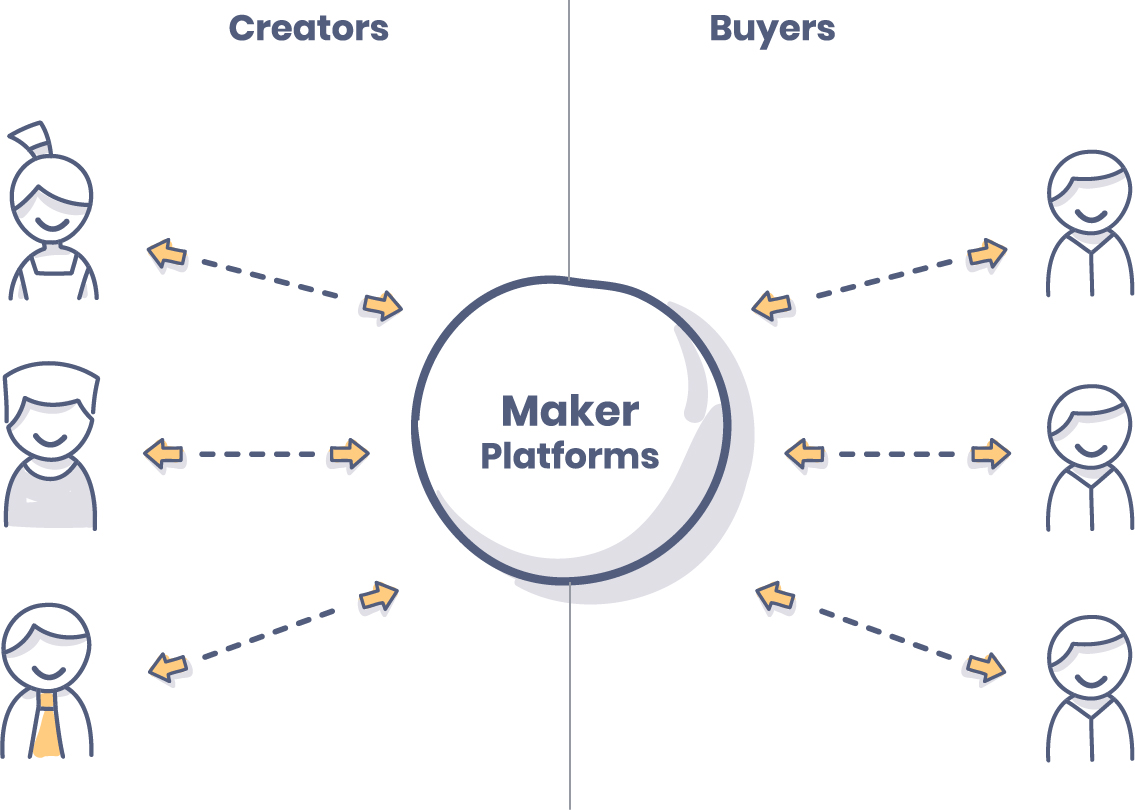
\includegraphics[width=.8\linewidth]{./figures/fig9.jpg}
  \caption{Maker Platforms.}
  \label{fig:maker}
\end{minipage}
\begin{minipage}{.45\textwidth}
  \centering
  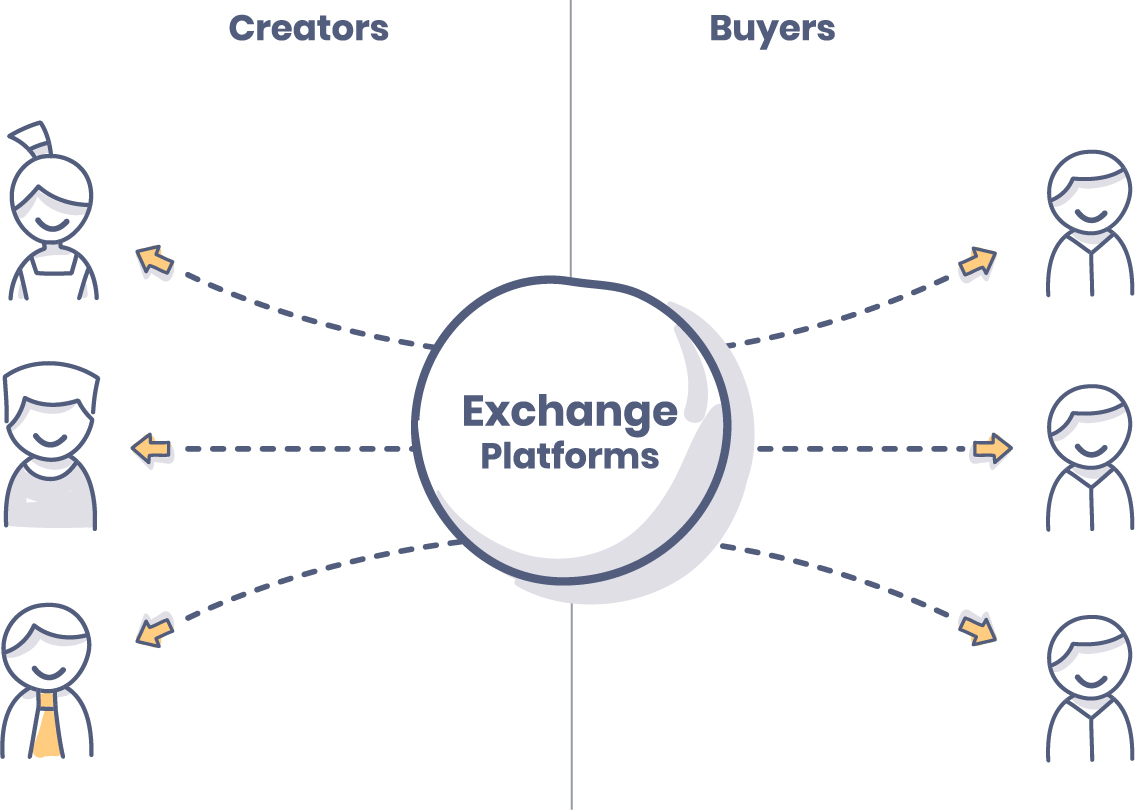
\includegraphics[width=.8\linewidth]{./figures/fig10.jpg}
  \caption{Exchange Platforms.}
  \label{fig:exchange}
\end{minipage}%
\end{figure}
 
\subsection{Sustainability}

A solid and growing community is paramount to the BlockLicense success. Like any other innovation, a certain time will be needed before it penetrates the market.  The adoption period, for new technologies, looks like an ‘S’ curve \cite{pierre}, as shown in Figure \ref{fig:scurve}, where customer segmentation is spread among five main categories: innovators, early adopters, early majority, late majority and laggards.

Once the crowdfunding campaign starts 
It is expected that on pre-, on and post-launch period, BlockLicense will gain market momentum, forming a noteworthy community of innovators and early adopters that will later expand to include early and late majority members. 

With an aim of achieving a 3\% of market share by the sixth year of  BlockLicense's operation, it is fundamental that  continuous marketing activities take place that focus on bringing additional value to the Blocklicense community. Activities may include incentives for both creators and buyers to use the ecosystem such as, \textit{bonus schemes} and \textit{ambassador programs} to name a few. Yet alone, marketing activities and incentives are not capable of growing or even maintaining the community. BlockLicense aims to constantly improve and expand the ecosystem by looking at the community needs.

\begin{figure}[h]
\centering
\begin{minipage}{1\textwidth}
  \centering
  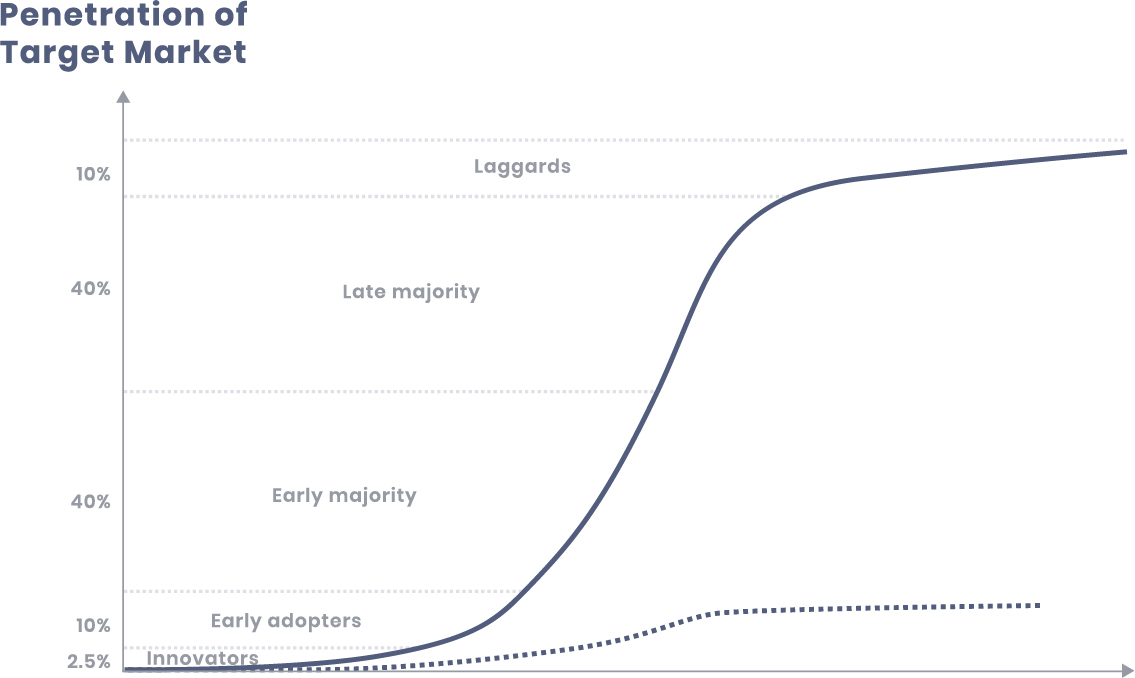
\includegraphics[width=.8\linewidth]{./figures/fig11.jpg}
  \caption{Market Penetration.}
  \label{fig:scurve}
\end{minipage}
\end{figure}
\newpage
\section{CROWDSALE} \label{crowdsale}

In order to raise funds and kickstart the BlockLicense Ecosystem development, we will be running a crowdfunding campaign during which LCN will be exchanged for ETHER. The campaign will run in two stages over a period of \textit{12 weeks}. As we can see in Table \ref{table:coindistribution}, a total of \textit{700,000,000LCN} will be issued at a price of \textit{2,000LCN per ETH}. During Stage 1 of crowdfunding \textit{5\%} of the total LCN will be made available for purchase, while during Stage 2, \textit{65\%} of the total LCN will be made available. 
\newline
\bigskip
BlockLabs will reserve the remaining \textit{30\%} of the total LCN issued to cover:

\begin{itemize}
\item -- Bounty Tokens
\item -- Crowdsale Bonuses
\item -- Market Liquidity (if needed)
\item -- BlockLicense needs
\end{itemize}

After the end of the crowdsale campaign (Stages 1 \& 2) all unsold LCN from the pool of LCN available during the campaign will be burned and LCN will be listed in several crypto exchanges to be traded at will.
\newline
\bigskip
Funds raised during the crowdsale will be used to cover costs in the following areas:

\begin{itemize}
\item \textbf{Marketing:} - Advertising, press releases, videos, social media etc
\item \textbf{Capital:} - Funds available as working capital for BlockLicense
\item \textbf{Security:} - Security auditing and fortification of payment processing EVM code
\item \textbf{Founders:} - The founders fee
\item \textbf{Legal:} - BlockLicense legal costs
\item \textbf{Sundry:} - Unpredicted expenses associated with product development and launch
\item \textbf{Support:} - Funds provided to external partners
\end{itemize}

In the sections that follow we analyze each crowdfunding stage carefully and show that funds raised serve vital needs of the BlockLicense project.


\begin{table}[t]
\begin{center}
\begin{tabular}{c c c c c}
& & \\ % put some space after the caption
\toprule
\textbf{LCN Issued} & \textbf{ETH Rate} & \textbf{BlockLabs Reserve}  & \textbf{Stage 1: Presale} & \textbf{Stage 2: ICO} \\
\midrule
700,000,000 & 2,000 LCN for 1 ETH & 30\% & 5\% & 65\% \\
\bottomrule
\end{tabular}
\end{center}
\caption{LCN Distribution}
\label{table:coindistribution}
\end{table}



\subsection{Stage 1: Presale}


During this stage we aim to raise funds that will be used to cover initial expenses related to the BlockLicense project. These include vital costs such as security auditing of our smart contract code, marketing \& promotional costs associated with making the BlockLicense project known to a wider audience and supporting Stage 2 of our crowdfunding campaign.


\begin{itemize}
\item --- Any remaining LCN from the Presale stage will be added to the pool of LCN available during Stage 2: ICO.
\item --- In case the project doesn't reach its minimum target, any funds raised during the presale stage are non-refundable. 
\end{itemize}

Presale will run over a period of 4 weeks and bonus LCN will be given to contributors as shown in Table \ref{presale-bonus}:

\begin{table}[h]
\centering
\begin{tabular}{@{}lclll@{}}
\toprule
& \textbf{Week 1} & \multicolumn{1}{c}{\textbf{Week 2}} & \multicolumn{1}{c}{\textbf{Week 3}} & \multicolumn{1}{c}{\textbf{Week 4}} \\ 
\midrule
\multicolumn{1}{r}{\textbf{Bonus}} & 30\%            & 30\%                                & 25\%                                & 25\%   \\ 
\bottomrule
\end{tabular}
\caption{Presale Bonus LCN}
\label{presale-bonus}
\end{table}

The allocation of Ether raised during Presale depends on the total sum raised. The first 100ETH raised will be allocated and used as described in Table \ref{presale-fund-a}. 
\bigskip
% Please add the following required packages to your document preamble:
% \usepackage{booktabs}
\begin{table}[h]
\centering
\begin{tabular}{@{}lccccccc@{}}
\toprule
& \textbf{Marketing} & \textbf{Security} & \textbf{Capital} & \textbf{Founders} & \textbf{Legal} & \textbf{Sundry} & \textbf{Support} \\ 
\midrule
\multicolumn{1}{r}{\textbf{Fund Allocation}} & 65\%               & 35\%              & 0\%              & 0\%               & 0\%            & 0\%             & 0\%              \\ 
\bottomrule
\end{tabular}
\caption{Allocation of Presale funds for the first 100ETH raised}
\label{presale-fund-a}
\end{table}

\bigskip
Any Ether raised during Presale above the sum of 100 ETH will be allocated and used as described in Table \ref{presale-fund-b}: 
\begin{table}[h]
\centering
\begin{tabular}{@{}lccccccc@{}}
\toprule
& \textbf{Marketing} & \textbf{Security} & \textbf{Capital} & \textbf{Founders} & \textbf{Legal} & \textbf{Sundry} & \textbf{Support} \\ 
\midrule
\multicolumn{1}{r}{\textbf{Fund Allocation}} & 55\%               & 10\%              & 20\%              & 10\%               & 2\%            & 1\%             & 2\%              \\ 
\bottomrule
\end{tabular}
\caption{Allocation of Presale funds raised above 100ETH }
\label{presale-fund-b}
\end{table}

\newpage

\subsection{Stage 2: ICO}
This is the main stage of our crowdfunding campaign that will determine the fate of the BlockLicense project.

ICO will run over a period of 6 weeks and bonus coins will be distributed as described in Table \ref{ico-bonus}:


\begin{table}[h]
\centering
\begin{tabular}{@{}lllllll@{}}
\toprule
               & \textbf{Week 1}          & \textbf{Week 2}          & \textbf{Week 3}          & \textbf{Week 4}          & \textbf{Week 5}          & \textbf{Week 6}          \\ \midrule
\textbf{Bonus} & \multicolumn{1}{c}{20\%} & \multicolumn{1}{c}{20\%} & \multicolumn{1}{c}{15\%} & \multicolumn{1}{c}{15\%} & \multicolumn{1}{c}{15\%} & \multicolumn{1}{c}{15\%} \\ \bottomrule
\end{tabular}
\caption{ICO Bonus LCN}
\label{ico-bonus}
\end{table}

\bigskip

Funds raised during the ICO will be allocated as described in Table \ref{ico-fund}:
\begin{table}[h]
\centering
\begin{tabular}{@{}lccccccc@{}}
\toprule
& \textbf{Marketing} & \textbf{Security} & \textbf{Capital} & \textbf{Founders} & \textbf{Legal} & \textbf{Sundry} & \textbf{Support} \\ 
\midrule
\multicolumn{1}{r}{\textbf{Fund Allocation}} & 30\%               & 1\%              & 40\%              & 25\%               & 1\%            & 2\%             & 1\%              \\ 
\bottomrule
\end{tabular}
\caption{Allocation of ICO funds }
\label{ico-fund}
\end{table}



\subsection{Minimum Goals}

The sustainability of the BlockLicense project depends on the amount of ETH that will be raised during the crowdsale campaign. A high enough sum guarantees that there are enough funds to create the BlockLicense Ecosystem in its entirety, while a low sum will prevent the project from continuing. In the latter case, funds raised during Stage 2 will be refundable, while funds raised during Stage 1 will be non-refundable. 

\begin{multicols}{2}
\begin{equation} \label{eq:goalA}
  \operatorname{MinGoalA} =
  \begin{cases}
    1,000\operatorname{ETH} & \text{if 1 ETH $\geq$ \$250} \\
     2,000\operatorname{ETH} & \text{otherwise}
  \end{cases}
\end{equation}\break
\begin{equation} \label{eq:goalB}
  \operatorname{MinGoalB} =
  \begin{cases}
    5,000\operatorname{ETH} & \text{if 1 ETH $\geq$ \$250} \\
     10,000\operatorname{ETH} & \text{otherwise}
  \end{cases}
\end{equation}
\end{multicols}



There are two minimum crowdfunding goals that we have set for BlockLicense, namely MinGoalA (\ref{eq:goalA}) and MinGoalB (\ref{eq:goalB}). If MinGoalA fails, the project will not continue. If MinGoalA succeeds while MinGoalB fails, we will use raised funds to build the Desktop Application. If MinGoalB succeeds, we will use raised funds to create the entire Ecosystem.
\newpage
\section{TEAM} \label{team}
\bigskip
\noindent
\textbf{Nikolas Psaroudakis} \newline
\medskip Founder, Technical Director
\newline
Nikolas is a multidisciplinary developer and maker. Driven by his innate curiosity, he enjoys finding out how things work. He views code as an expressive medium and excels in producing technological solutions for forward looking businesses and individuals. He has been educated in two continents and has lived and worked in four countries. He holds a BSc in Physics, an MSc in the area of Computer Vision and an MPS in Interactive Telecommunications. Nikolas is a firm believer in the potential of the decentralized web as an agent for change and the positive impact blockchain \& Web 3.0 can have on the society as a whole.\par

%%%%%%%%%%%%%%%%%%%%%%%%%%%%%%%%%%%%%%%%%%%%%%%%%%%%%
\bigskip
\noindent
\textbf{Katerina Stavraki}\newline
\medskip Cofounder, Business Director
\newline
Katerina is a multi-skilled corporate mind with over 15 years of experience in B2B and B2C multinational corporations. She holds a BEng in Communications Engineering and an MSc in Electrical Power Engineering and Management from top institutions in the UK. Katerina is effective and efficient and believes in TRN, short for Technology-Resolution-Now. Her unique project management skills gained her experience in diverse fields such as business development and planning as well as strategic projects across several countries in the world. Katerina is a blockchain enthusiast \& investor and believes in technological revolution behind the numbers.\par


%%%%%%%%%%%%%%%%%%%%%%%%%%%%%%%%%%%%%%%%%%%%%%%%%%%%%
\bigskip
\noindent
\textbf{Yiannis Koutsoupas}\newline
\medskip Cofounder, Art Director
\newline
Yiannis is a designer at heart and practice, a problem solver and UX/UI expert; his experience spans from websites to apps since 2000. Yannis’s portfolio of collaborators includes agencies, global corporations \& innovative startups among others. His creative portfolio holds innovative projects, nominated and award winning projects in the realms of broadcasting, advertising and disruptive technological programs.
 \par

%%%%%%%%%%%%%%%%%%%%%%%%%%%%%%%%%%%%%%%%%%%%%%%%%%%%%
\bigskip
\noindent
\textbf{Theodore Moulos}\newline
\medskip Cofounder, Growth Strategist
\newline
Theodore is a Growth-Hacking Strategist. He has been on the game for over 15 years during which he has won over intrapreneurship and entrepreneurship. Having conquered all types of positions (CEO, COO, BoD member, etc.) within international companies (e.g. Pinnatta App) he now goes by ‘Theodore’ and during his free time, he coaches startups. He is the owner of GrowthRocks and Viral-Loops companies, taming digital marketing practices.
\par
%%%%%%%%%%%%%%%%%%%%%%%%%%%%%%%%%%%%%%%%%%%%%%%%%%%%%
\bigskip
\noindent
\textbf{Jason Kritikos}\newline
\medskip iOS \& Backend Developer
\newline
Jason is an iOS addict and a restless coder. Holding a BSc in Computer Science and a master’s degree in mobile \& wireless networks, Jason has proven early his passion for anything mobile. Having worked in London and Athens for more than 15 years, he’s gained significant experience in building anything from backend systems to mobile apps for both large corporations and innovative startups. He enjoys spinning records and shooting with his camera.
\par

%%%%%%%%%%%%%%%%%%%%%%%%%%%%%%%%%%%%%%%%%%%%%%%%%%%%%
\bigskip
\noindent
\textbf{Alex Galinos}\newline
\medskip Business Advisor
\newline 
Alex is a Harvard Business School graduate determined to offer experience and expertise to his country. More specifically by holding, throughout his career, managing positions in the Hellenic Ministry of Foreign Affairs, the Athens Development and Destination Management Agency and the Athens City Hall. As a professional, Alex is a firm believer and, thus, invests in business extroversion and openness.
\par
%%%%%%%%%%%%%%%%%%%%%%%%%%%%%%%%%%%%%%%%%%%%%%%%%%%%%
\bigskip
\noindent
\textbf{Konstantina Chardalia}\newline
\medskip Financial Advisor
\newline
Konstantina is a finance mastermind using her devotion to numbers and her loyalty to forecasting and planning for the greater balance. She graduated from top universities in Greece and the UK and established herself as a professional expert in Greece. Konstantina’s experience in multinational corporations and her consistency in growing and evolving make her a uniquely gifted partner.
\par
%%%%%%%%%%%%%%%%%%%%%%%%%%%%%%%%%%%%%%%%%%%%%%%%%%%%%
\bigskip
\noindent
\textbf{Sofia Stavraki}\newline
\medskip Legal Advisor
\newline
Sofia is a Supreme Court lawyer. She is a Democritus University of Thrace Alumna who practices Criminal \& Trade Law, Civil Law and issues Legal agreements from her private law firm/office of 2 branches, in Lamia and Athens, Greece, owned since 2002 \& 2011 accordingly. Sofia is an avid writer and reader manifested in her rich professional website, in her published law essays and her 500+ wins in Greek courts until today.
\par

%%%%%%%%%%%%%%%%%%%%%%%%%%%%%%%%%%%%%%%%%%%%%%%%%%%%%
\bigskip
\noindent
\textbf{Olga Kachramanoglou}\newline
\medskip Copywriter \& Social Media 
\newline
Olga is a loyal writer. She identifies herself as an anthropologist but writing is her moneymaker. From advertising copywriter-before the digital Big Bang-to content creator she never stops to write for the digital market (SEO, social media \& blogging) and for fun. She was once labeled handicap for her wild imagination in writing. However, she is, still, fully functional and social but would rather write to you than speak to you.
 \par
\newpage
\bibliographystyle{asmems4}
\bibliography{whitepaper}
\end{document}